\documentclass[11pt]{article}
\usepackage[margin=1in]{geometry}
\usepackage{amsmath,amssymb,booktabs,graphicx,authblk,siunitx,microtype}
\usepackage[hidelinks]{hyperref}
\graphicspath{{figs/}}

% ============================================================
% SKELETON ONLY -- 6 numbered sections. [..] = thesis/placeholder.
% Target: arXiv math.NA/cs.NA -> J. Comput. Phys. / J. Sci. Comput.
% ============================================================

\title{On the Sensitivity of Shock-Capturing PINN Benchmarks\\
to Reference Resolution}
\author[1]{Abdelhalim Azzouz}
\affil[1]{Department of Mathematics, University of Naama, Algeria}
\date{}

\begin{document}
\maketitle

\begin{abstract}
Geometry-aligned collocation, which concentrates a physics-informed neural
network's training points near a shock, is an appealing remedy for the
under-resolution of discontinuities. We show that its apparent success can be an
artifact of the reference solver used to score it. On inviscid Burgers on the
torus, a Bernstein collocation sampler beats uniform and residual-adaptive
baselines in the mean on all three metrics---on all ten seeds for the shock and
global errors (eight of ten for the smooth region), by up to $26\%$ on the shock
metric at $p\approx10^{-3}$---when graded against a first-order reference; the same trained models, graded
against a second-order reference \emph{on the same grid}, lose every metric by
$19$--$43\%$. The advantage correlates ($+0.79$) with reference front width: it
exists only insofar as the reference is under-resolved. We trace the mechanism to
the concentration of an ill-posed strong-form residual on the singular set, which
over-diffuses the front; a second, compressible-Euler case fails by a distinct
amplitude-bias mechanism. We give a simple differential test---re-score fixed
checkpoints against references of increasing fidelity---that detects the confound
in any shock benchmark.
\end{abstract}

% ===== 1 ====================================================
\section{Introduction}\label{sec:intro}
% PINNs under-resolve shocks; strong-form residual ill-posed at discontinuities
% [De Ryck-Mishra, Krishnapriyan, Fuks-Tchelepi]. Collocation strategies (RAR,
% geometry-aligned, gPINN). QUESTION: does geometry-aligned collocation improve
% shock capture? FINDING (up front): the apparent gain is a reference artifact.
Physics-informed neural networks (PINNs) solve PDEs by minimizing a residual
loss on collocation points~\cite{Raissi2019}. For nonlinear hyperbolic
conservation laws the approach is strained at its core: shocks occupy a vanishing
fraction of the domain yet dominate the error, and the strong-form residual is
ill-posed at a genuine discontinuity, where the flux derivative is distributional.
Minimizing it provably need not select the entropy solution and tends toward
smooth approximants that miss the front~\cite{DeRyckMishra2024,Krishnapriyan2021,
Fuks2020}. Localized artificial-viscosity remedies act on the operator to restore well-posedness~\cite{Coutinho2023}; geometry-aligned sampling, by contrast, leaves the loss unchanged and merely relocates where it is enforced. A natural response is to change \emph{where} the residual is enforced:
residual-adaptive refinement~\cite{Lu2021}, gradient-enhanced
losses~\cite{Yu2022}, and geometry-aligned samplers that concentrate collocation
near the shock all aim to spend the training budget where it matters.

This paper asks a narrow question about one such strategy---geometry-aligned
Bernstein collocation, which draws points from a tube around the shock
manifold---and arrives at a cautionary, general answer. Measured against a
first-order finite-volume reference, the method shows a large, clean,
statistically robust shock-capture advantage: it attains the lowest mean error on
all three metrics, winning on all ten seeds in the shock and global errors (eight
of ten in the smooth region), by up to $26\%$ on the shock metric at
$p\approx10^{-3}$. Yet the same trained models, scored
against a faithful second-order reference \emph{on the same grid}, lose every
metric by $19$--$43\%$. The advantage is not a property of the method; it is a
property of the reference solver. The apparent gain is a reference-resolution
artifact, and the strong-form pathology above is precisely its mechanism: the
sampler concentrates an ill-posed loss on the singular set, producing a more
diffuse solution that only \emph{appears} better when graded against a blurry
answer key.

We do not claim that geometry-aligned collocation, or the field's benchmarks at
large, are uniformly flawed---high-fidelity references (WENO, exact Riemann
solvers) are common, and we survey no prevalence. We claim something narrower and
verifiable: that a standard validation protocol can manufacture a spurious method
ranking, that the effect is mechanistic and reproducible, and that a simple test
detects it.
\paragraph{Contributions.}
\begin{enumerate}
  \item A demonstrated case in which reducing reference resolution \emph{inverts} the measured method ranking, with the trained models held fixed.
  \item A reusable \emph{differential reference test}---re-score fixed checkpoints against references of increasing fidelity---that detects the artifact in any shock benchmark.
  \item An identification of the mechanism (front over-diffusion from concentrating an ill-posed strong-form residual on the singular set), anchored in existing hyperbolic ill-posedness theory.
  \item A second, system (Euler) case in which geometry-aligned collocation underperforms uniform sampling through a \emph{distinct} mechanism (amplitude bias, not diffusion), refuting the approach along an independent axis.
\end{enumerate}

% ===== 2 ====================================================
\section{Method under test and protocol}\label{sec:protocol}
% Geo-Bernstein sampling (uniform + Bernstein/Beta tube around prescribed front).
% Strong-form residual loss; Fourier embedding; architecture. Burgers 2D torus; IC.
% CRITICAL LEVER: two reference solvers -- 1st-order Rusanov vs MUSCL+minmod.
% Shock mask (90th-pct gradient); metrics (global/shock/smooth L1).
\textbf{Method.} Geo-Bernstein leaves the architecture, loss, optimizer, point
budget, and training length of a standard PINN unchanged; it alters only the PDE
collocation distribution. After a uniform warm-up, points are drawn from a mixture
$\mu = \alpha\,\mu_{\mathrm{unif}} + (1-\alpha)\,\mu_{\mathrm{front}}$, where
$\mu_{\mathrm{front}}$ samples a tube of width $\tau$ around the prescribed shock
manifold with a symmetric Bernstein/Beta offset kernel; a curriculum tightens
$(\alpha,\tau)$ during training. The loss is the standard strong form,
$\mathcal{L}=\frac1{N_f}\sum_i|\mathcal{R}_\theta(x_i)|^2
+\lambda_{\mathrm{IC}}\,\mathcal{L}_{\mathrm{IC}}$, identical across methods.

\textbf{Benchmark.} The primary problem is inviscid Burgers on $\mathbb{T}^2$,
$u_t+\partial_x(u^2/2)+\partial_y(a\,u^2/2)=0$ with $a=0.5$, horizon $T=0.25$, and
a straight periodic front of Rankine--Hugoniot speed; periodicity is enforced by a
Fourier embedding, so no boundary loss is needed. Baselines are Vanilla (uniform)
and residual-adaptive refinement (RAR) under the identical loss and protocol.

\textbf{References and metrics.} The discontinuity is scored against two
finite-volume references on a common grid: a first-order Rusanov solver~\cite{Rusanov1961} and a
second-order MUSCL scheme with a minmod limiter~\cite{vanLeer1979}. The shock mask is the set of
cells above the $90$th percentile of the reference density gradient; we report the
$L^1$ error globally, on the mask (shock), and off the mask (smooth). The choice of
reference solver---not of method---is the variable interrogated in
Section~\ref{sec:reversal}.
\begin{table}[t]\centering
\caption{Common training protocol (10 seeds).}\label{tab:protocol}
\begin{tabular}{ll}\toprule
Quantity & Value \\ \midrule
$N_f=8000$, $N_{IC}=2048$, steps $=3500$, warm-up $=1000$ & \\
Network & 5-layer MLP, width 96, $\tanh$, Fourier input \\
Learning rate / clip / optimizer & $10^{-3}\!\to\!5\times10^{-4}$ / 10 / Adam \\
Seeds & $0,1,\dots,9$ \\
Reference solvers & first-order Rusanov \emph{vs.} MUSCL+minmod (2nd order) \\
\bottomrule
\end{tabular}
\end{table}

% ===== 3 (merge: apparent result + reversal) ================
\section{The apparent result and its reversal}\label{sec:reversal}
\subsection{The apparent result}\label{sec:apparent}
% "What an ordinary paper would publish": vs 1st-order 160^2, Geo wins all metrics,
% 10/10, +19.6/+25.8% shock, p<1e-3. Reproducible, clean, and misleading.
Trained under the protocol of Section~\ref{sec:protocol} and evaluated against
the first-order Rusanov reference on a $160\times160$ grid, Geo-Bernstein attains
the lowest mean error on all three metrics (Table~\ref{tab:apparent}). The
shock-region improvement over Vanilla is $19.6\%$ ($25.8\%$ over RAR), with a
$9.2\%$ global and $5.1\%$ smooth-region gain. The effect is not marginal: a
one-sided Wilcoxon signed-rank test on the per-seed shock error rejects equality
at the floor of its $10$-seed support, $p=2^{-10}\approx 9.8\times10^{-4}$, with
Geo-Bernstein lower in the shock region on \emph{all ten} seeds against both
baselines (the global metric is likewise $10/10$; the smooth region is $8/10$ vs
Vanilla, $9/10$ vs RAR). Taken at face
value, this is a clean, reproducible, statistically significant result of exactly
the kind that ordinarily warrants publication. The remainder of the paper shows
that it is an artifact of the reference solver.
\begin{table}[t]\centering
\caption{Burgers $\mathbb{T}^2$, vs first-order $160^2$ reference (10 seeds). Geo wins all metrics.}\label{tab:apparent}
\begin{tabular}{lccc}\toprule
Method & Global $L^1$ & Shock $L^1$ & Smooth $L^1$ \\ \midrule
Vanilla & 0.02336 & 0.06630 & 0.01859 \\
RAR & 0.02430 & 0.07181 & 0.01903 \\
Geo-Bernstein & \textbf{0.02121} & \textbf{0.05329} & \textbf{0.01765} \\
\bottomrule
\end{tabular}
\end{table}

\subsection{The differential test}\label{sec:differential}
% Same trained models; change ONLY the reference.
% Cleanest control: same grid 160^2, scheme only -> flip from +9/+20/+5% (10/10)
% to -25/-43/-19% (0/10). Battery over 6 references -> Geo loses 0-2/10 by 15-43%.
% FIGURE R1: gain vs reference front width, corr +0.79.
The trained networks are fixed; only the object they are \emph{compared
against} changes. We therefore re-evaluate the same checkpoints against
references of increasing fidelity, holding the grid, mask definition, and metric
identical. The cleanest control fixes the grid at $160\times160$ and changes only
the scheme, from first-order Rusanov to second-order MUSCL with a minmod limiter.
Under this single change the verdict inverts: Geo-Bernstein moves from leading
on all three metrics in the mean ($+9.2/+19.6/+5.1\%$; $10/10$ seeds on the global
and shock errors, $8/10$ on the smooth) to \emph{trailing} on all three on
essentially every seed ($-25.4/-43.3/-18.8\%$; $0/10$, $0/10$, $1/10$). No resolution change is involved;
only the accuracy of the reference front.

Extending this to a battery of six references (Table~\ref{tab:battery}) confirms
that the reversal is neither a MUSCL artifact nor a single-resolution accident: a
first-order reference at $320^2$ already suffices to collapse the advantage
($2/10$), and every sharper reference, first- or second-order, places
Geo-Bernstein behind Vanilla by $15$--$43\%$ on the shock metric. The harness is
validated by its exact reproduction of Table~\ref{tab:apparent} against the
original $160^2$ first-order reference. Figure~\ref{fig:r1} summarizes the
mechanism in one curve: the Geo-Bernstein shock advantage is a monotone,
strongly positive function of the reference front width (correlation $+0.79$),
i.e.\ it exists \emph{only} to the extent that the reference is under-resolved. A
faithful reference removes it entirely.
\begin{table}[t]\centering
\caption{Same models, varying the reference: Geo shock gain vs Vanilla flips sign as the reference sharpens.}\label{tab:battery}
\begin{tabular}{lcc}\toprule
Reference & Geo vs Vanilla & Shock gain \\ \midrule
1st-order $160^2$ (paper) & 10/10 & $+19.6\%$ \\
1st-order $320^2$ & 2/10 & $-28.9\%$ \\
1st-order $640^2$ & 2/10 & $-17.8\%$ \\
MUSCL $256^2$ & 0/10 & $-27.2\%$ \\
MUSCL $384^2$ & 0/10 & $-21.6\%$ \\
MUSCL $512^2$ & 0/10 & $-17.5\%$ \\
\bottomrule
\end{tabular}
\end{table}
\begin{figure}[t]\centering
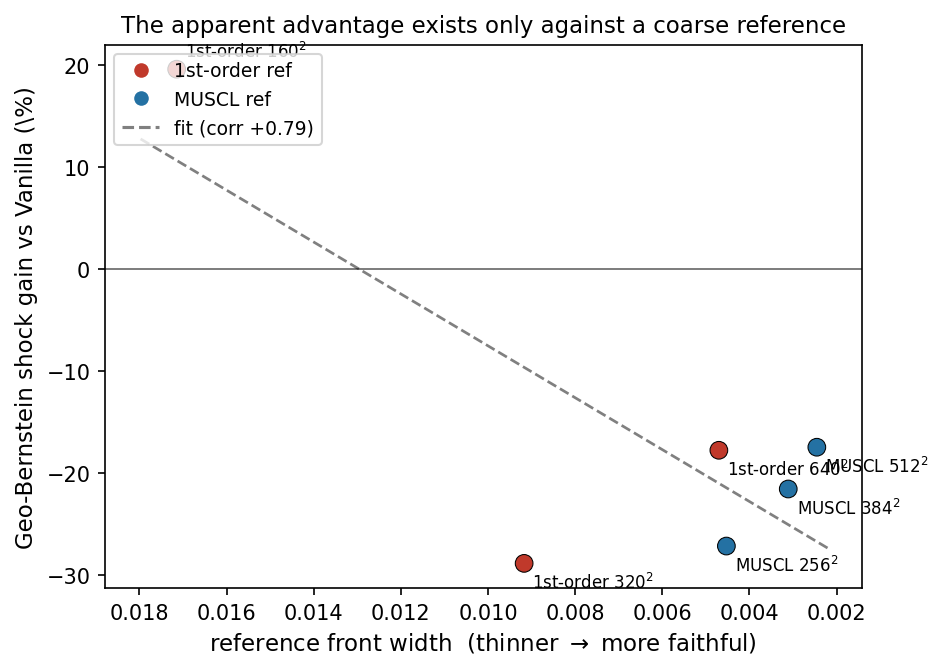
\includegraphics[width=0.66\linewidth]{r1_gain_vs_reference_width.png}
\caption{The apparent advantage is a decreasing function of reference quality (corr $+0.79$).}\label{fig:r1}
\end{figure}

% ===== 4 (merge: both mechanisms) ===========================
\section{Mechanisms of failure}\label{sec:mech}
\subsection{Scalar Burgers: front over-diffusion}\label{sec:mech-burgers}
% H1: Geo front 4.8x wider than MUSCL ref vs 2.5x Vanilla (max|grad| 27/52/129).
% H2 ruled out (centered, XI~-0.001). H4 ruled out (sampler works, 3.4x enrichment).
% R2: per-seed corr(diffusion, error)=+0.60. Anchor: strong-form ill-posed at shock.
Why does correctly concentrating collocation at the front make the solution
worse? We isolate the cause on the scalar benchmark through three diagnostics on
the trained models, evaluated against the MUSCL $384^2$ reference.

\emph{H1 (front sharpness).} Measured by the peak density-gradient magnitude, the
reference front has $\max|\nabla u|\approx 129$; Vanilla reaches $52$ (a front
$2.5\times$ wider than the reference) while Geo-Bernstein reaches only $27$, a
front $4.8\times$ wider. Geo-Bernstein produces the \emph{most diffuse} solution
of the three (Figure~\ref{fig:burgers-err}): its error is a smooth halo straddling
the front, not a localized defect.

\emph{H2 and H4 (ruled out).} The over-diffusion is neither a misplaced front nor a
sampler bug. The Geo-Bernstein front is centred on the true front to within
$\xi\approx-1.4\times10^{-3}$ (versus $-3\times10^{-5}$ for Vanilla), excluding a
shock-speed drift; and the front-aligned sampler does its job, enriching the
shock band by $3.4\times$ over uniform sampling. The geometry is transmitted to
the point set exactly as designed---the failure lies downstream of the sampler.

\emph{R2 (diffusion controls the error).} Across the ten seeds, a network's
front diffusion predicts its shock error: the per-seed correlation between front
width and shock $L^1$ is $+0.60$. The same correlation holds for Vanilla, so
``more diffuse $\Rightarrow$ larger error'' is a general law; H1 supplies the
missing piece, namely that Geo-Bernstein is the method that diffuses most.

These assemble into a single causal chain. The strong-form residual
$|\mathcal{R}_\theta|^2$ is ill-posed at a genuine discontinuity, where the flux
derivative is distributional rather than pointwise; minimizing it does not select
the entropy solution and, as established analytically for hyperbolic problems,
drives the network toward smooth approximants that miss the
shock~\cite{DeRyckMishra2024}. Geo-Bernstein concentrates the training budget
precisely on this ill-posed region. The sampler thus amplifies, rather than
mitigates, the strong-form pathology: it sharpens \emph{where} the loss is least
valid, yielding a globally smoother and less accurate solution. Against an
under-resolved reference---itself a diffuse front---this extra smoothing is
invisible or even flattering; against a faithful reference it is exposed as a net
loss on every metric.
\begin{figure}[t]\centering
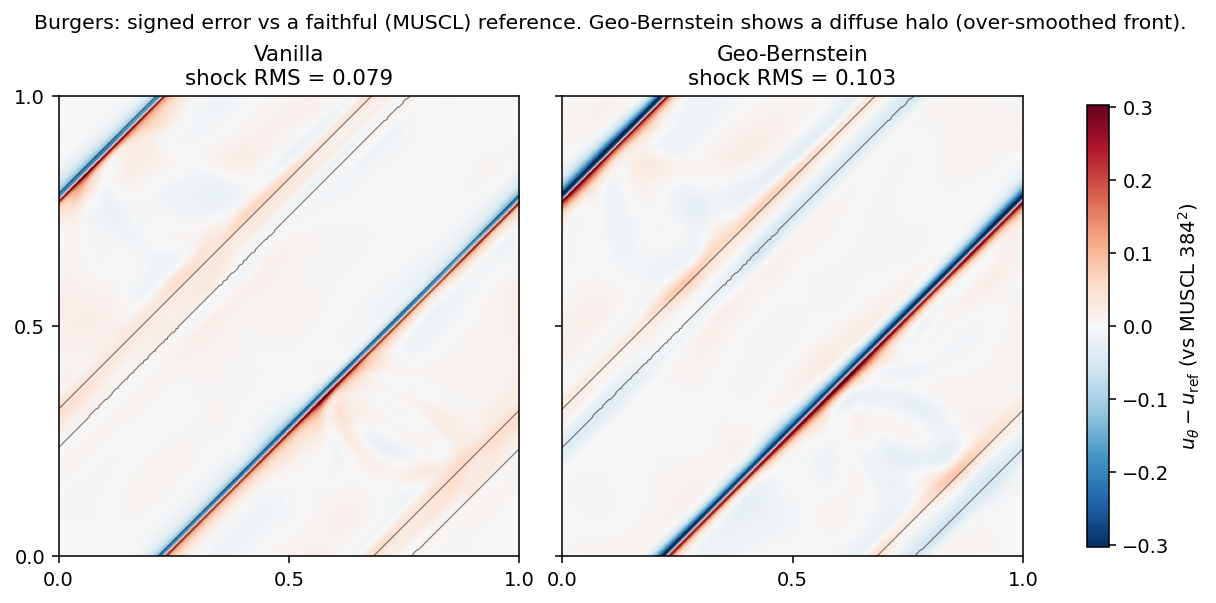
\includegraphics[width=0.74\linewidth]{signed_error_maps_burgers.png}
\caption{Burgers, signed error vs MUSCL $384^2$ (seed 0, illustrative). Geo shows a diffuse halo: an over-smoothed front ($4.8\times$ reference width). Quantitative claims use the 10-seed statistics of Sec.~\ref{sec:differential}.}\label{fig:burgers-err}
\end{figure}

\subsection{System Euler: amplitude bias}\label{sec:mech-euler}
% HONEST LABEL: optimized variant (Bernstein-OPT, width 72, 5 seeds), related
% two-front Euler. Bernstein loses to Vanilla on ALL metrics on the run's OWN ref.
% DISTINCT mechanism: fronts equally sharp (56.5/54.9/53.7); error uncorrelated
% with Laplacian (~0.07); failure = amplitude under-shoot (~80% of error energy).
We now ask whether the same mechanism governs a system. The case we can examine
with saved checkpoints is an \emph{optimized} Bernstein-collocation variant
(here ``Bernstein-OPT'', width $72$, five seeds) on a related two-front
compressible Euler problem; it is not the network of Table~\ref{tab:apparent},
and we treat it only as an independent system data point. On this problem the
geometric sampler again fails to help---but for a different reason, and without
any need to sharpen the reference.

Against the run's own reference, plain Vanilla wins \emph{every} metric
(Table~\ref{tab:euler}): Bernstein-OPT is $29\%$ worse on the shock density error
and $40\%$ worse globally. Crucially, this is \emph{not} the Burgers
over-diffusion mechanism. The predicted fronts are as sharp as the reference
($\max|\nabla\rho|$ of $56.5$ for Bernstein-OPT, $54.9$ for Vanilla, $53.7$ for
the reference; Figure~\ref{fig:euler-err}, bottom), so the front is neither
smeared nor mislocated. Instead the signed density error is a systematic
\emph{amplitude bias}: every method under-shoots the density jump, with a net
shock-band bias that accounts for roughly $80\%$ of the error energy and is
uncorrelated with the reference Laplacian (correlation $\approx 0.07$, excluding a
diffusion signature). Geo-Bernstein worsens this bias rather than correcting it
(net bias $-0.26$ versus $-0.19$ for Vanilla).

The two cases therefore expose two distinct failure modes of geometry-aligned
collocation: front over-diffusion in the scalar problem, and amplitude bias in
the system. They share a single conclusion---concentrating a strong-form residual
on the singular set does not improve, and can degrade, shock-region accuracy---but
they refute the method along independent axes, which is harder to dismiss than a
single mechanism observed twice.
\begin{figure}[t]\centering
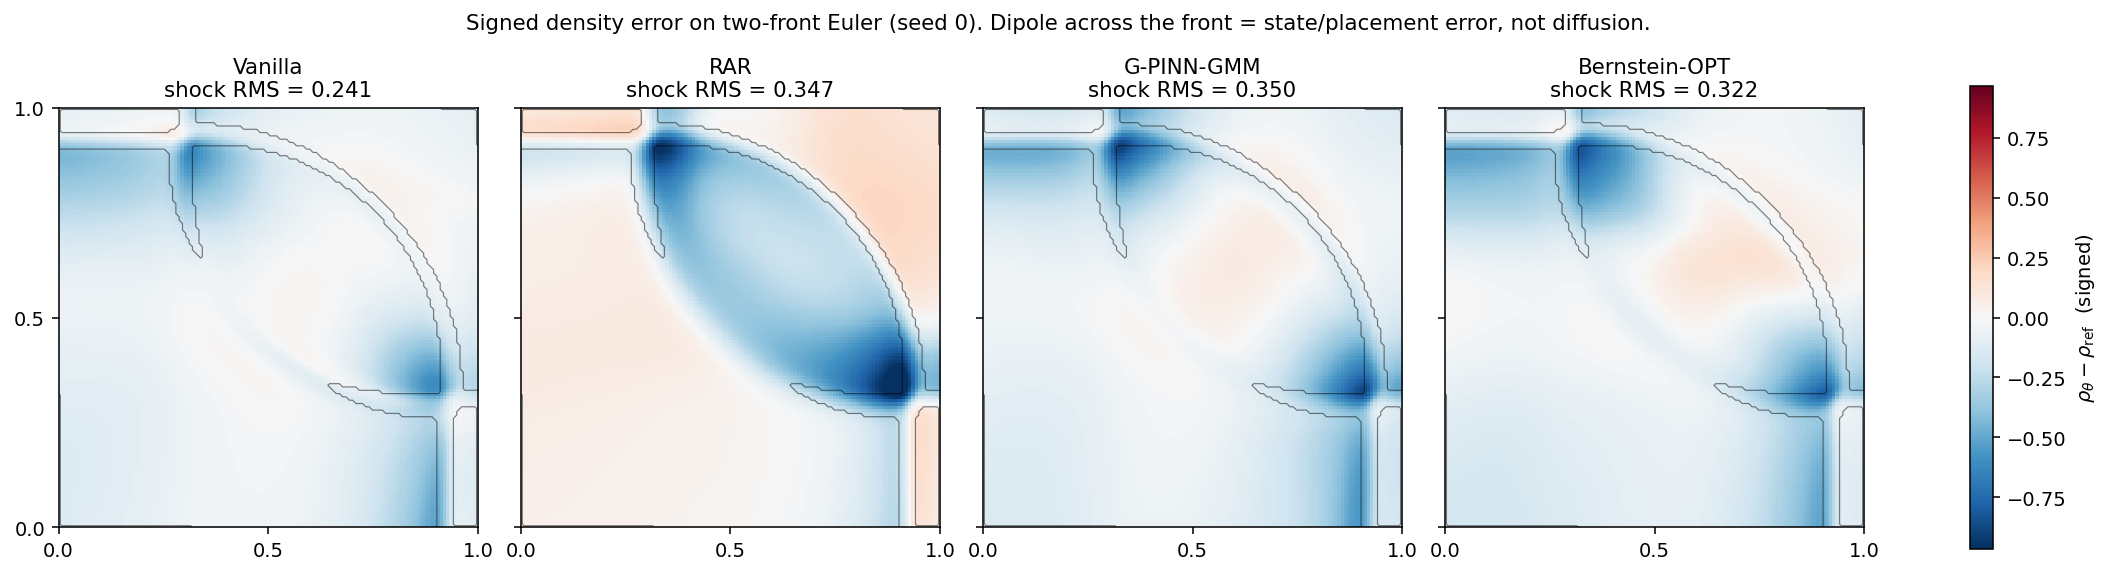
\includegraphics[width=0.92\linewidth]{signed_error_maps_euler.png}\\[2pt]
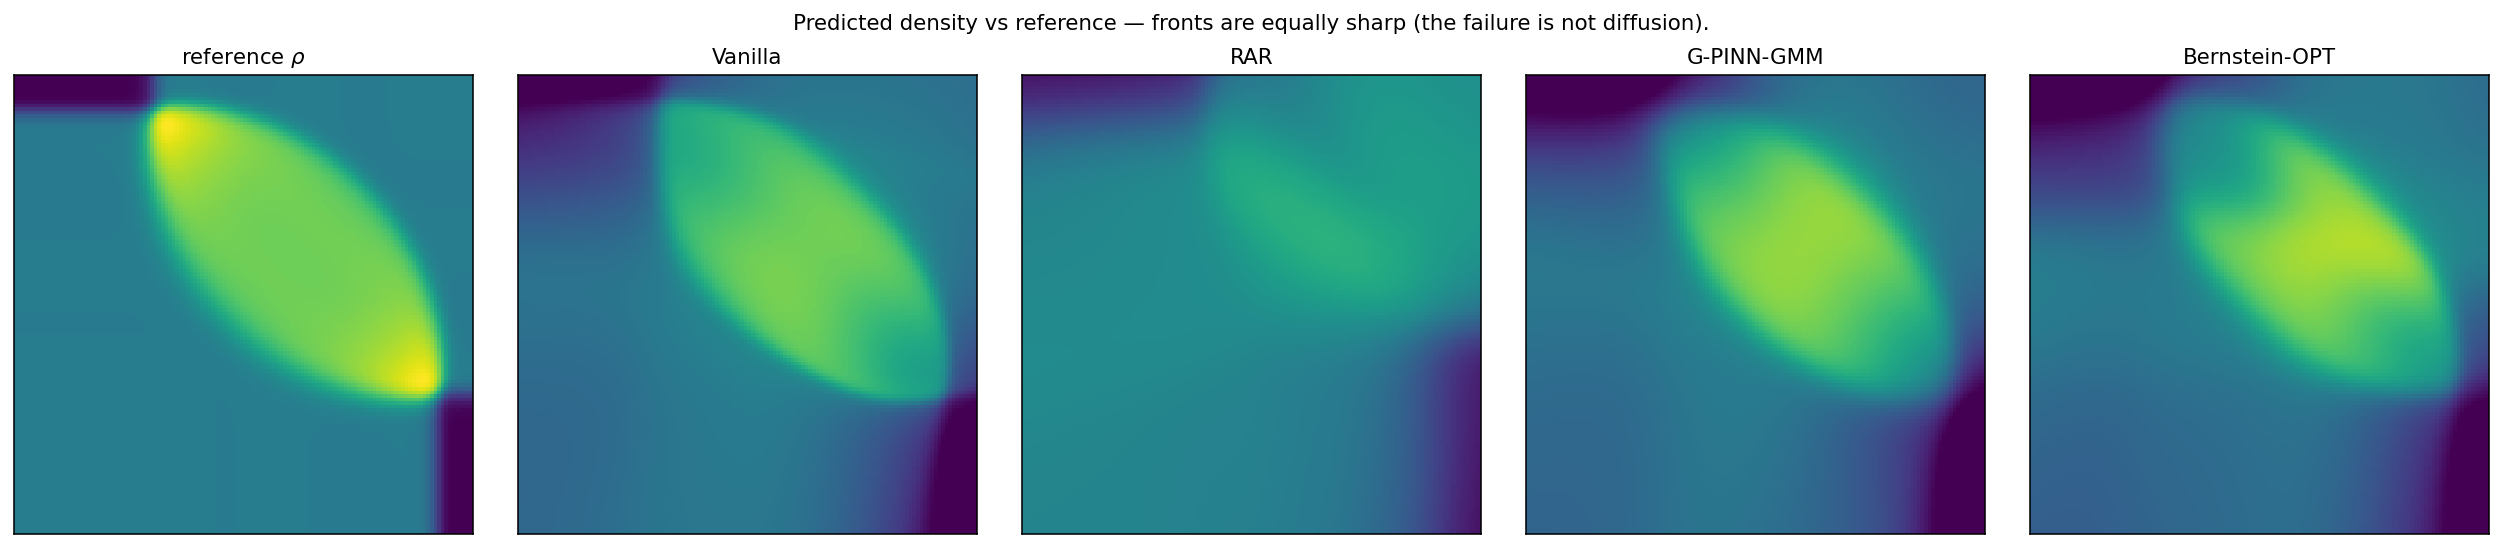
\includegraphics[width=0.92\linewidth]{predicted_rho_euler.png}
\caption{Two-front Euler (seed 0, illustrative). Top: signed density error -- an amplitude bias (systematic under-shoot), not a diffuse halo. Bottom: predicted vs reference density -- fronts equally sharp, so the mechanism differs from Burgers.}\label{fig:euler-err}
\end{figure}
\begin{table}[t]\centering
\caption{Two-front Euler (Bernstein-OPT variant, 5 seeds). Vanilla wins every metric.}\label{tab:euler}
\begin{tabular}{lcccc}\toprule
Method & $\rho\,L^1$ & shock $\rho\,L^1$ & front recall & front prec. \\ \midrule
Vanilla & \textbf{0.1072} & \textbf{0.2315} & 0.4375 & 0.4771 \\
RAR & 0.1762 & 0.3172 & 0.3562 & 0.3884 \\
G-PINN-GMM & 0.1464 & 0.3194 & 0.4344 & 0.4736 \\
Bernstein-OPT & 0.1497 & 0.2990 & 0.4229 & 0.4611 \\
\bottomrule
\end{tabular}
\end{table}

% ===== 5 (implications + limitations) =======================
\section{Implications, recommendations, and limitations}\label{sec:implications}
% Differential test as a tool. Use references with a reported convergence study
% (WENO / MUSCL / exact Riemann). HONEST SCOPE: vulnerability + demonstrated case,
% NOT a prevalence survey or a claim the field is broadly wrong.
The practical lesson is procedural, not specific to one sampler. Because the
trained models are independent of the reference, a method's ranking can be made to
flip by changing the yardstick alone; any shock benchmark that scores against a
single, unvalidated reference is exposed to the same confound. We therefore
recommend two safeguards. First, validate against references with a reported
convergence study---WENO~\cite{JiangShu1996}, MUSCL, or exact Riemann solutions---rather than a
first-order solver of convenience. Second, apply the \emph{differential test} of
Section~\ref{sec:reversal}: re-score the fixed checkpoints against at least one
sharper reference and confirm that the ranking is stable. The test is nearly free,
requires no retraining, and would have caught the artifact reported here before
submission.

We make no claim about prevalence. High-fidelity references are common in the
shock-capturing PINN literature, and we have surveyed none systematically; our
contribution is a demonstrated mechanism and a detection tool, not an indictment
of the field.
\paragraph{Limitations.}
% strong-form loss only; prescribed front; Euler = optimized variant (width 72,
% 5 seeds, distinct mechanism, not the original Table-4 model); viscous regime
% excluded (null); no prevalence claim.
Our analysis concerns the strong-form residual; we make no claim about
weak-form or variational PINNs, for which the singular-set pathology may not
apply. The Burgers front geometry is prescribed rather than learned. The Euler
case is an optimized variant (width $72$, five seeds) on a related setup with a
distinct failure mechanism, and is not the scalar model of
Table~\ref{tab:apparent}. The viscous regime, where the front is genuinely smooth
and the strong-form residual well-posed, is excluded as it yields a null result
(all methods tied within seed noise).

% ===== 6 ====================================================
\section{Conclusion}\label{sec:conclusion}
% Collocation design has confounds; reference resolution can invert rankings.
% Two distinct failure modes. Validate against faithful references; apply the test.
Collocation design is not a free lunch, and its evaluation is not confound-free.
A geometry-aligned sampler that appears to deliver a large, statistically robust
shock-capture gain is shown to owe that gain entirely to an under-resolved
reference; against a faithful reference on the same grid it loses on every metric.
The same family of methods fails on a compressible-Euler system through a second,
distinct mechanism. The constructive takeaways are simple: score shock benchmarks
against references whose resolution has been verified, and apply a differential
reference test---which costs no retraining---before trusting a reported ranking.

\paragraph{Code and data availability.}
% GitHub: load_pt.py (loads checkpoints without torch), step0.py (MUSCL ref +
% battery), r1r2.py (R1/R2), heatmaps*.py; checkpoints + config; README mapping
% each command to a table/figure.
All results are reproducible from saved checkpoints. The repository provides
\texttt{load\_pt.py} (loads checkpoints without a deep-learning runtime),
\texttt{step0.py} (MUSCL reference and the six-reference battery),
\texttt{r1r2.py} (the gain--width and diffusion--error analyses), and the figure
scripts, together with the checkpoints, configuration, and a README mapping each
command to a table or figure.

\begin{thebibliography}{99}
\bibitem{Raissi2019} M. Raissi, P. Perdikaris, G.E. Karniadakis, Physics-informed neural networks: a deep learning framework for solving forward and inverse problems involving nonlinear PDEs, J. Comput. Phys. 378 (2019) 686--707.
\bibitem{Lu2021} L. Lu, X. Meng, Z. Mao, G.E. Karniadakis, DeepXDE: a deep learning library for solving differential equations, SIAM Rev. 63 (2021) 208--228.
\bibitem{Yu2022} J. Yu, L. Lu, X. Meng, G.E. Karniadakis, Gradient-enhanced physics-informed neural networks for forward and inverse PDE problems, Comput. Methods Appl. Mech. Engrg. 393 (2022) 114823.
\bibitem{DeRyckMishra2024} T. De Ryck, S. Mishra, Improving weak PINNs for hyperbolic conservation laws, arXiv:2211.12393v2, 2024.
\bibitem{Krishnapriyan2021} A.S. Krishnapriyan, A. Gholami, S. Zhe, R.M. Kirby, M.W. Mahoney, Characterizing possible failure modes in physics-informed neural networks, Adv. Neural Inf. Process. Syst. 34 (2021) 26548--26560.
\bibitem{Fuks2020} O. Fuks, H.A. Tchelepi, Limitations of physics informed machine learning for nonlinear two-phase transport in porous media, J. Mach. Learn. Model. Comput. 1 (2020) 19--37.
\bibitem{Coutinho2023} E.J.R. Coutinho, M. Dall'Aqua, E. Gildin et al., Physics-informed neural networks with adaptive localized artificial viscosity, arXiv:2203.08802, 2022.
\bibitem{vanLeer1979} B. van Leer, Towards the ultimate conservative difference scheme. V, J. Comput. Phys. 32 (1979) 101--136.
\bibitem{JiangShu1996} G.-S. Jiang, C.-W. Shu, Efficient implementation of weighted ENO schemes, J. Comput. Phys. 126 (1996) 202--228.
\bibitem{Rusanov1961} V.V. Rusanov, Calculation of interaction of non-steady shock waves with obstacles, J. Comput. Math. Math. Phys. USSR 1 (1961) 267--279.
\end{thebibliography}

\end{document}
